\section{Task 1}

\begin{question}
    Design the data warehouse to address the specifications and to efficiently answer to all
    the provided frequent queries.
    Draw the conceptual schema of the data warehouse and the logical schema (fact and dimension tables).
\end{question}
\begin{answer}
    \subsection{Conceptual Design}
    \\
    \begin{center}
        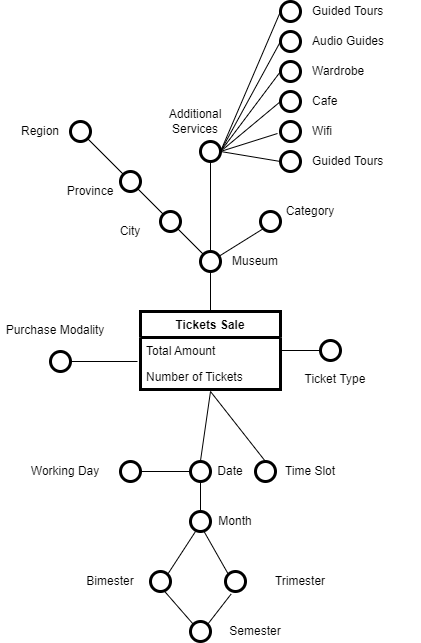
\includegraphics[width=0.9\textwidth]{01DWDesign.png}
        \captionof{figure}{Data Warehouse Conceptual Design}
    \end{center}
    \pagebreak
    \subsection{Logical Design}
    \underline{Primary keys are underlined}
    \subsubsection{Facts}
    The only fact table is the tickets sale which will be determined by the total amount and the number of tickets.
    The purchase modality, ticket type, and time slot are added into this table given that there are not many features
    for this dimensions.The only special attribute on TIME is slot that can contain a number from 1 to 3
    for each of the three blocks(08:00-12:00, 12:01-16:00, 16:01- 20:00)
    \par
    \textbf{TICKETSALE}(\underline{timeID, museumID}, totalAmount, numberOfTickets, purchaseModality, ticketType,
        timeSlot)
    \subsubsection{Dimensions}
    The dimensions are timeDim and museum. The museum dimension contains every one of the additional services as a binary
    column. This decision is taken on the fact that the number of services is known and not greater than 10, so it would
    help us to avoid an extra join or multiple records. The sub dimension LOCATION also was extracted, so that the same
    location can be used more than one time, and we do not overpopulate the MUSEUM table.
    \par
    \textbf{TIMEDIM}(\underline{timeID}, validDate, month, bimester, trimester, semester, workingDay, holiday) \\
    \textbf{MUSEUM}(\underline{museumID}, museumName, locationID, name, category, guidedTours, audioGuides, Wardrobe, Cafe,
    Wifi) \\
    \textbf{LOCATION}(\underline{locationID}, city, province, region) \\
\end{answer}
\pagebreak
